\documentclass[border=5pt]{standalone}
\usepackage{tikz}

\newcommand{\carpet}[4]{%
  \ifnum#4=0
    \fill (#1,#2) rectangle ++(#3,#3);
  \else
    \pgfmathsetmacro{\s}{#3/3}
    \pgfmathtruncatemacro{\next}{#4-1}
    \foreach \dx/\dy in {0/0,1/0,2/0,0/1,2/1,0/2,1/2,2/2}{
      \pgfmathsetmacro{\nx}{#1+\dx*\s}
      \pgfmathsetmacro{\ny}{#2+\dy*\s}
      \carpet{\nx}{\ny}{\s}{\next}
    }
  \fi
}

\begin{document}
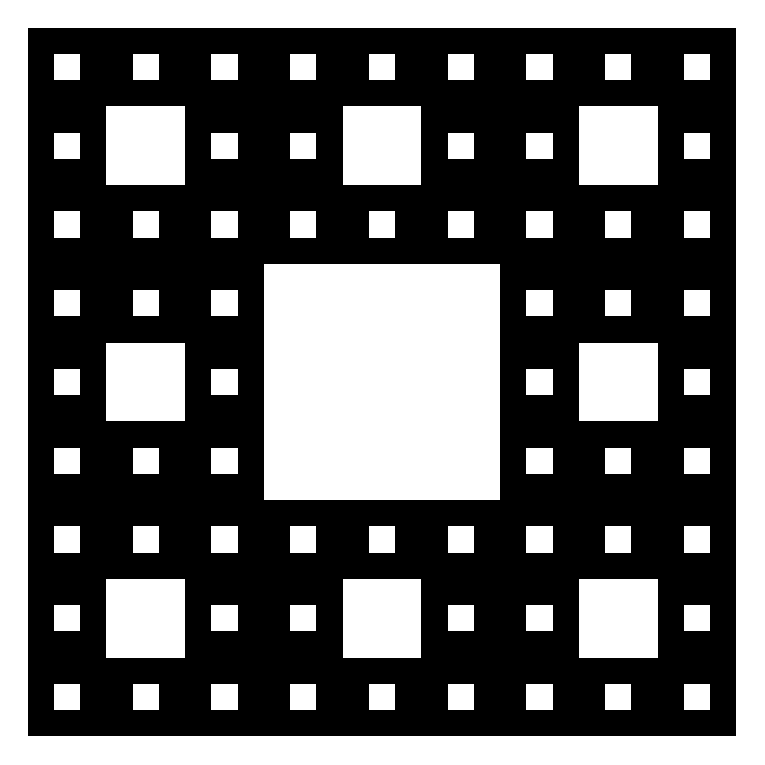
\begin{tikzpicture}
  \carpet{0}{0}{9}{3}
\end{tikzpicture}
\end{document}
